\hypertarget{a00330}{}\section{A\+A\+X communication protocols}
\label{a00330}\index{A\+A\+X communication protocols@{A\+A\+X communication protocols}}
How to transfer data between different parts of an A\+A\+X plug-\/in. 

A\+A\+X is a highly modular architecture. This section describes the various means by which A\+A\+X plug-\/in modules may communicate with one another and with the host.

There are two fundamental categories of communication in \hyperlink{a00288}{A\+A\+X}\+:
\begin{DoxyEnumerate}
\item \hyperlink{a00330_CommonInterface_Communication_hostmodules}{Communication with the C++ interface objects}
\item \hyperlink{a00330_CommonInterface_Communication_algorithm}{Communication with the real-\/time algorithm}
\end{DoxyEnumerate}\hypertarget{a00330_CommonInterface_Communication_hostmodules}{}\subsection{Communication with the C++ interface objects}\label{a00330_CommonInterface_Communication_hostmodules}
\hypertarget{a00330_CommonInterface_Communication_hostmodules_controller}{}\subsubsection{Direct host communication}\label{a00330_CommonInterface_Communication_hostmodules_controller}
Most communication between the A\+A\+X host and the plug-\/in is accomplished via the \hyperlink{a00090}{A\+A\+X\+\_\+\+I\+Controller} interface. This interface contains methods for such things as\+:
\begin{DoxyItemize}
\item Retrieving environment information such as the current \hyperlink{a00090_afa1f9f64eeeab9570e5599f466fa699e}{sample rate}
\item Getting and setting Effect parameters such as the Effect\textquotesingle{}s \hyperlink{a00090_ad50aa6fd54e39623a58debd63d9551e1}{algorithmic delay}
\item Accessing host-\/managed information such as \hyperlink{a00337}{Plug-\/in meters} and M\+I\+D\+I
\item Accessing other host-\/managed communications protocols like \hyperlink{a00330_CommonInterface_Communication_algorithm_datapackets}{Data packets} and M\+I\+D\+I
\end{DoxyItemize}

In addition, the G\+U\+I uses a separate interface for managing view and event details with the host. This interface, \hyperlink{a00117}{A\+A\+X\+\_\+\+I\+View\+Container}, includes methods for\+:
\begin{DoxyItemize}
\item Retrieving information like the raw view and the currently held modifier keys
\item Requesting changes to view parameters (e.\+g. size)
\item Passing G\+U\+I events on to the host.
\begin{DoxyItemize}
\item This is an important function because the host may require its own specific behavior for certain events. For example, a command-\/control-\/option click in Pro Tools should bring up the parameter\textquotesingle{}s automation menu.
\end{DoxyItemize}
\end{DoxyItemize}\hypertarget{a00330_CommonInterface_Communication_hostmodules_customdata}{}\subsubsection{Custom data blocks}\label{a00330_CommonInterface_Communication_hostmodules_customdata}
Often it is necessary to transmit arbitrary blocks of custom plug-\/in data between different plug-\/in modules. In A\+A\+X, this is accomplished by \char`\"{}pushing\char`\"{} data to and \char`\"{}pulling\char`\"{} it from the plug-\/in\textquotesingle{}s \hyperlink{a00328}{data model}.

The abstract data model interface includes two custom data methods for this\+: \begin{DoxyItemize}
\item \hyperlink{a00061_a4728fcad006d921a07489144360f447e}{A\+A\+X\+\_\+\+I\+Effect\+Parameters\+::\+Get\+Custom\+Data()} \item \hyperlink{a00061_aa838cad04781853ef2e0b9df22a05170}{A\+A\+X\+\_\+\+I\+Effect\+Parameters\+::\+Set\+Custom\+Data()}\end{DoxyItemize}
It is the data model\textquotesingle{}s job to act as a go-\/between when custom data must be transmitted between a plug-\/in\textquotesingle{}s other modules.

For example, a plug-\/in may wish to send analysis data from its \hyperlink{a00333}{direct data module} to its \hyperlink{a00329}{G\+U\+I}. In this situation, the Direct Data object would call \hyperlink{a00061_aa838cad04781853ef2e0b9df22a05170}{Set\+Custom\+Data()} to update the data model whenever new data was available, while the G\+U\+I would \char`\"{}pull\char`\"{} the most up-\/to-\/date data via \hyperlink{a00061_a4728fcad006d921a07489144360f447e}{Get\+Custom\+Data()} whenever an update was required.

Note that the default implementations of these methods are empty and thus all implementation details, including thread safety guards, are left to the plug-\/in.\hypertarget{a00330_CommonInterface_Communication_hostmodules_notifications}{}\subsubsection{Notifications}\label{a00330_CommonInterface_Communication_hostmodules_notifications}
The \hyperlink{a00328}{data model} and \hyperlink{a00329}{G\+U\+I} interfaces include \hyperlink{a00061_aa3eaeb292d2ca84086a5a058171994fd}{notification hook} methods. These methods used for \hyperlink{a00206_afab5ea2cfd731fc8f163b6caa685406e}{host-\/to-\/\+Effect notifications} by default, but may also be called with custom notification I\+Ds in order to create custom notifications within a plug-\/in.\hypertarget{a00330_CommonInterface_Communication_hostmodules_directpointersharing}{}\subsubsection{Direct pointer sharing}\label{a00330_CommonInterface_Communication_hostmodules_directpointersharing}
If co-\/location is guaranteed, plug-\/in modules may directly share data pointers. For example, a non-\/real-\/time plug-\/in\textquotesingle{}s \hyperlink{a00334}{Host Processor} object may share a {\ttfamily this} pointer with its \hyperlink{a00328}{data model} object.

To guarantee co-\/location between modules that could normally be placed into different memory spaces by the host, use \char`\"{}constraint\char`\"{} properties\+:

\begin{DoxyItemize}
\item \hyperlink{a00283_a6571f4e41a5dd06e4067249228e2249ea79a0815fea6c8f1a0d8ed511aa88e9ff}{A\+A\+X\+\_\+e\+Property\+\_\+\+Constraint\+\_\+\+Location} \item \hyperlink{a00283_a6571f4e41a5dd06e4067249228e2249ea5d7fca796aba48b5dc364af0cc633a02}{A\+A\+X\+\_\+e\+Property\+\_\+\+Constraint\+\_\+\+Topology}\end{DoxyItemize}
To help avoid forwards-\/compatibility issues with future devices that support A\+A\+X, these constraints should be set whenever a plug-\/in requires co-\/location of its components. Note, however, that using a design that relies on co-\/location will prevent the plug-\/in from running in distributed environments and should therefore be avoided when possible.\hypertarget{a00330_CommonInterface_Communication_algorithm}{}\subsection{Communication with the real-\/time algorithm}\label{a00330_CommonInterface_Communication_algorithm}
An A\+A\+X plug-\/in\textquotesingle{}s algorithm is essentially a stateless callback and, therefore, all of its state data must at some level be managed by the host. This model is fundamentally different from the other plug-\/in modules, which are each objects with their own memory and state.

Most algorithmic data management is performed via the algorithm\textquotesingle{}s context structure. More information about memory management in A\+A\+X real-\/time algorithms can be found \hyperlink{a00327_alg_memmgmt}{here}.\hypertarget{a00330_CommonInterface_Communication_algorithm_datapackets}{}\subsubsection{Data packets}\label{a00330_CommonInterface_Communication_algorithm_datapackets}
The most common form of communication with a plug-\/in\textquotesingle{}s real-\/time algorithm callback is the transmission of read-\/only data from the data model to the context structure.

A\+A\+X includes a dedicated A\+P\+I for this task that provides buffered, optimized delivery of read-\/only data packets to the algorithm. For more information, see \hyperlink{a00327_alg_comm}{Communicating with the algorithm} .\hypertarget{a00330_CommonInterface_Communication_algorithm_fields}{}\subsubsection{Host-\/managed context fields}\label{a00330_CommonInterface_Communication_algorithm_fields}
Algorithms can also send data to the host and receive environment information through dedicated context fields. For example, the host can provide access to D\+M\+A facilities through an object accessed via a D\+M\+A field, and a plug-\/in can report meter values to the host via a dedicated meter field. For more information, see \hyperlink{a00327_alg_comm}{Communicating with the algorithm} .\hypertarget{a00330_CommonInterface_Communication_algorithm_directdata}{}\subsubsection{Direct data transfers}\label{a00330_CommonInterface_Communication_algorithm_directdata}
When other modules in the plug-\/in must interact directly with the algorithm\textquotesingle{}s state information this is accomplished via the \hyperlink{a00333}{Direct Data} interface. This interface provides an idle-\/time context in which the plug-\/in may read from or write to the algorithm\textquotesingle{}s private data memory. These transfers are unbuffered and therefore the plug-\/in must handle any appropriate thread-\/safety considerations. Collaboration diagram for A\+A\+X communication protocols\+:
\nopagebreak
\begin{figure}[H]
\begin{center}
\leavevmode
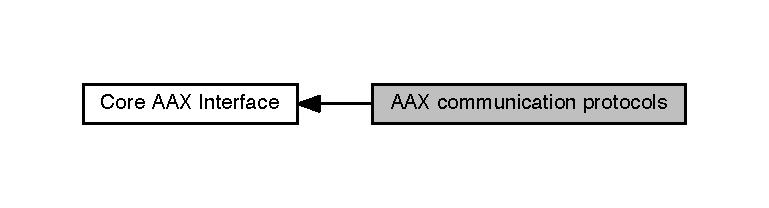
\includegraphics[width=350pt]{a00330}
\end{center}
\end{figure}
